\section{Day 4: Basis; Orderings on Sets; Product Topology (Sep. 12, 2024)}
Outfit of the day! Gives King Dice vibes tbh (from cuphead) i like the purple a lot :3
\begin{figure}[h]
    \centering
    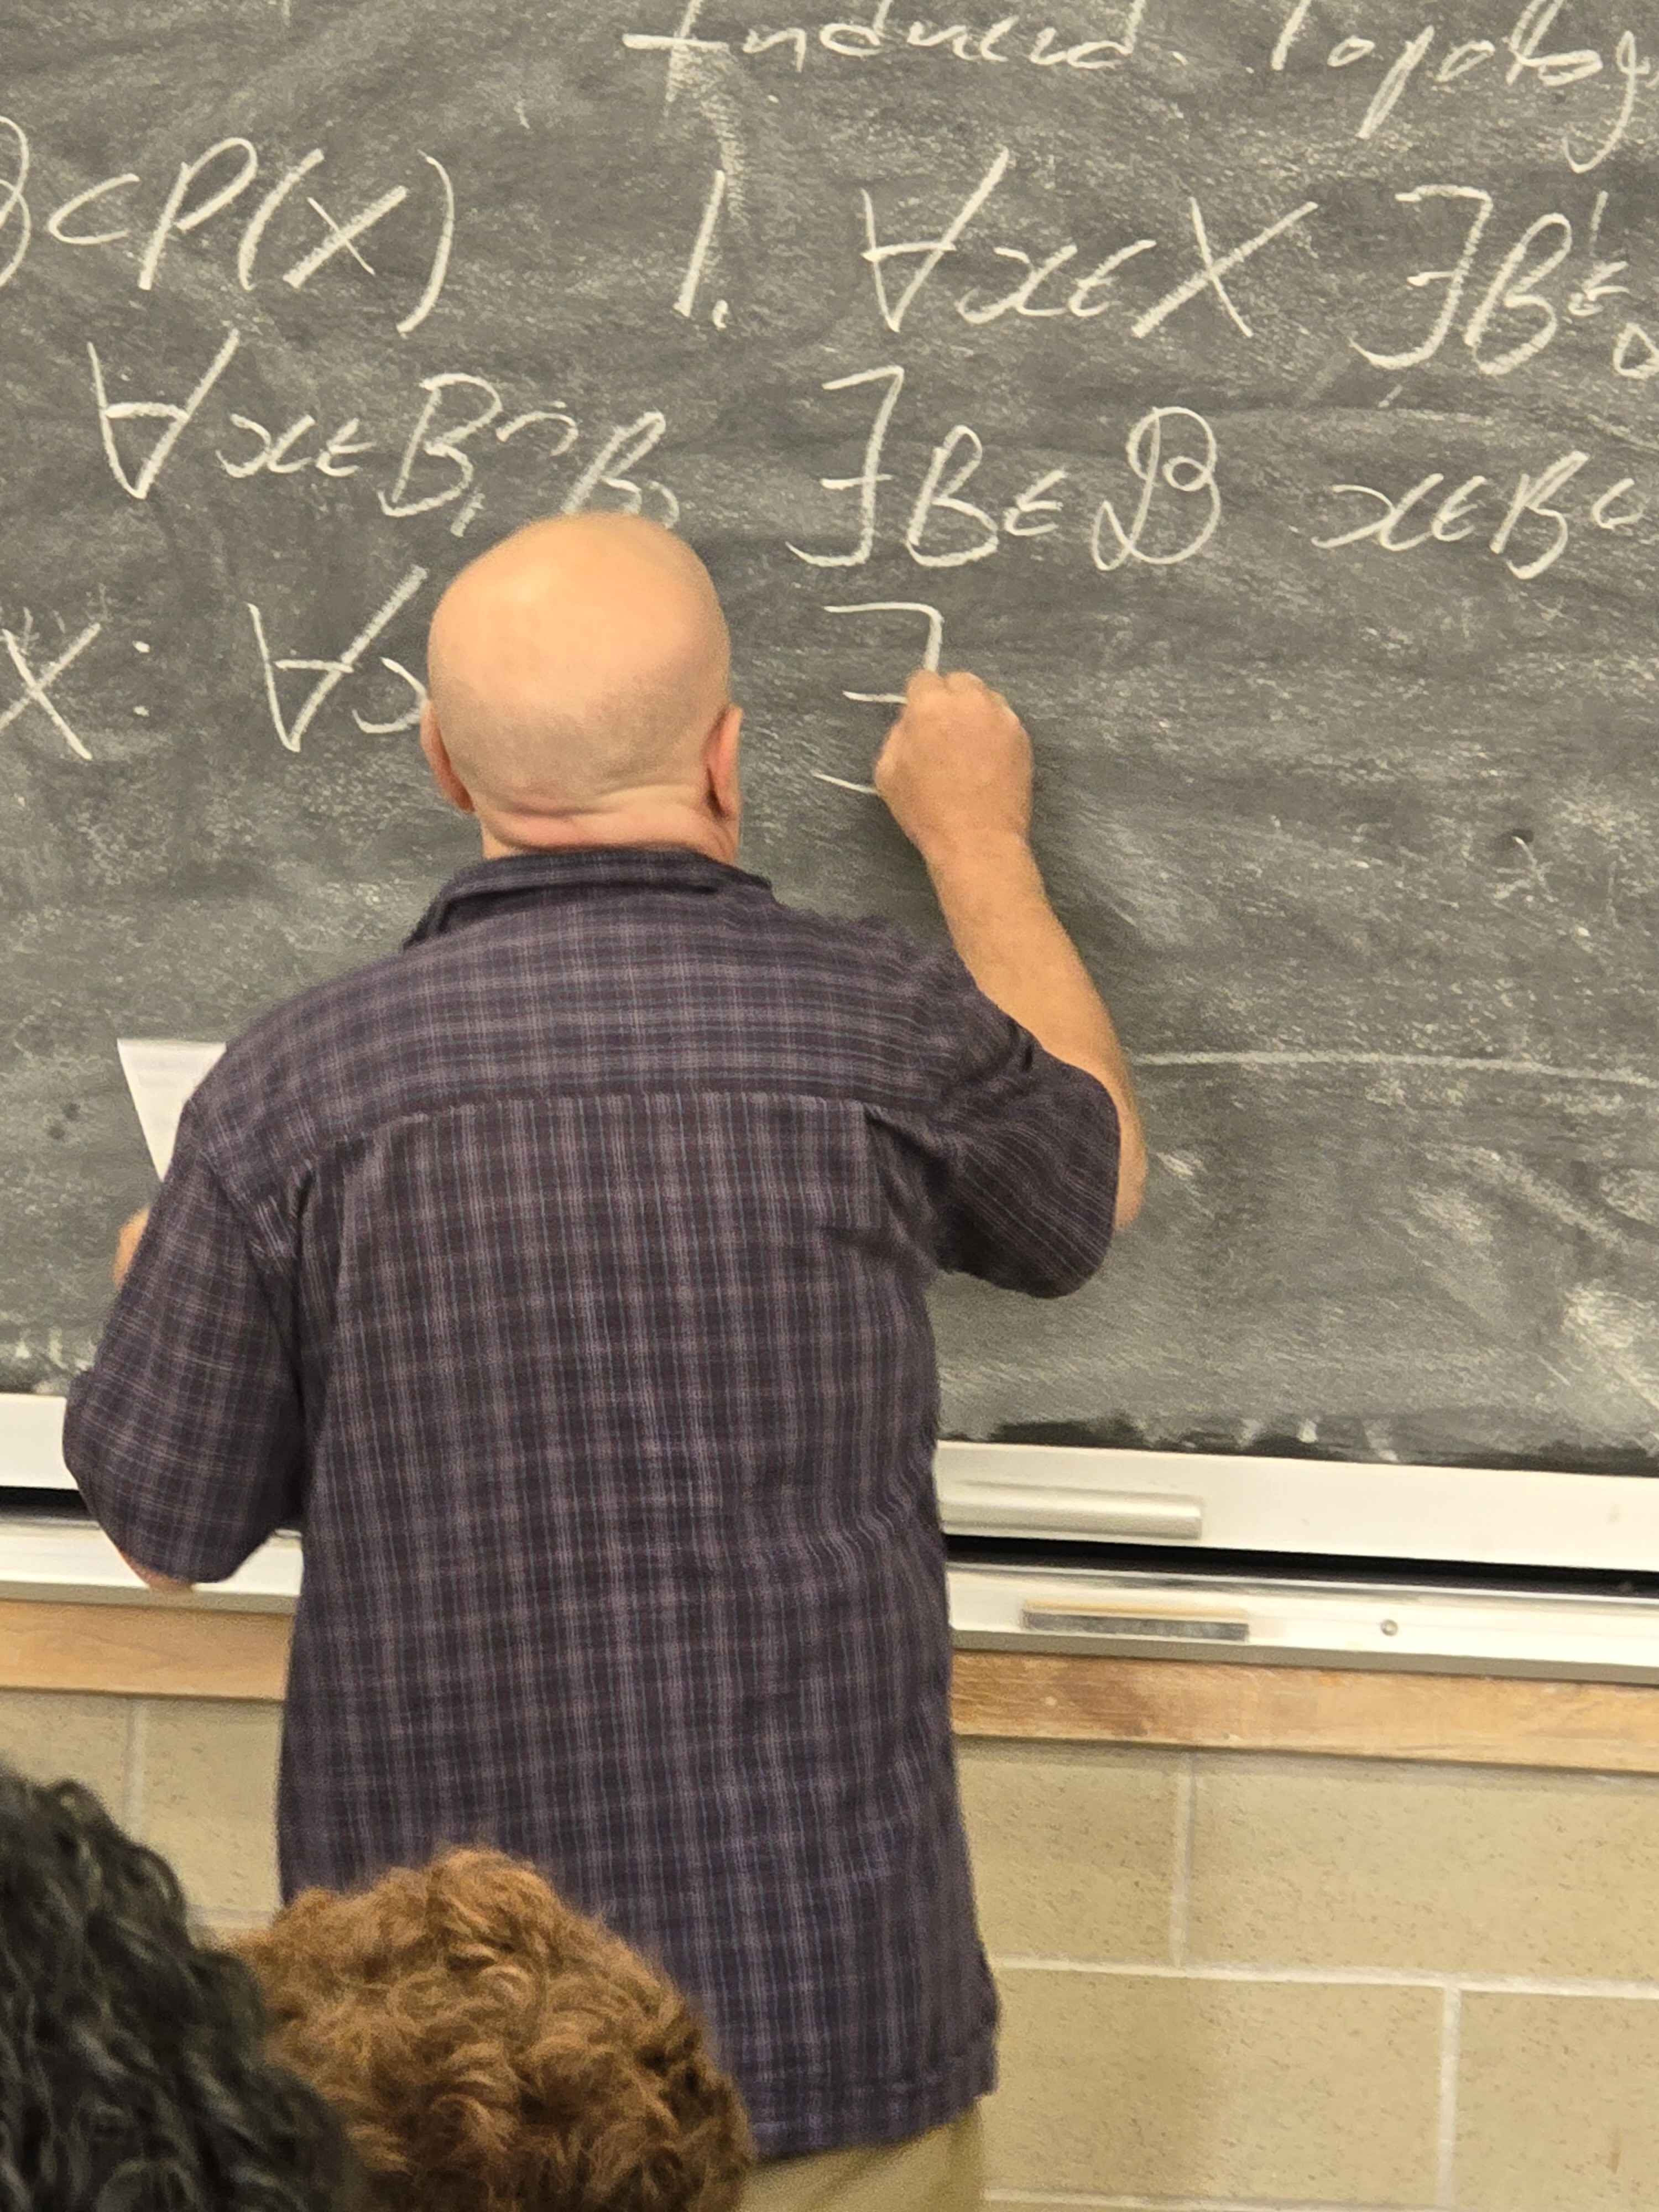
\includegraphics[scale=0.1]{MAT327 Notes/Dror Shirts/dror day 4 shirt.jpg}
\end{figure}

\noindent Recap of last lecture:
\begin{itemize}
    \item We define the basis $\SB \subset \SP(X)$ of a topology to have the following properties (which we will refer to as the first and second axioms),
    \begin{enumerate}
        \item For all $x \in X$, there exists a basic set $B \in \SB$ such that $x \in B$.
        \item For any $x$ in the intersection of two basic sets (i.e. $x \in B_1 \cap B_2$), there exists $B \in \SB$ such that $x \in B \subset B_1 \cap B_2$.
    \end{enumerate}
\end{itemize}
\noindent With this, we may construct the topology generated by $\SB$, i.e.
\[ \ST_\SB := \{ U \subset X \mid \forall x \in U, \exists B \in \SB \text{ s.t. } x \in B \subset U \}. \]

\newpage
\begin{simplethm}[Basis Topology is a Topology on $X$]
    We claim that $\ST_\SB$ is a topology on $X$.
\end{simplethm}
\noindent We proceed by checking that $\ST_\SB$ satisfies the required properties.
\begin{enumerate}
    \item Observe that $U = \emptyset, X$ are both in $\ST_\SB$; if $U = \emptyset$, then there are no elements $x \in U$ to bother about, of which the condition is vacuously true; if $U = X$, then the condition is true by the basis axioms.
    \item Let us consider an indexing set $I$, and let us consider the arbitrary union of subsets $U_\alpha \subset X$
    \[ U := \bigcup_{\alpha \in I} U_\alpha. \]
    Then any $x \in U$ belongs to $x \in U_\alpha$ for some index $\alpha \in I$; since $U_\alpha$ satisfies the condition, we see that the union $U$ also satisfies the condition as well.
    \item Finally, for intersections, let us take $U_1, U_2 \in \ST$ where\footnote{note that dror used superscript to separate the two types of base sets, but i'm going to subscript them in a list to keep it clear.}
    \begin{align*}
        U_1 &= \bigcup_{\alpha_1 \in A_1} B_{1, \alpha_1}, \\
        U_2 &= \bigcup_{\alpha_1 \in A_2} B_{2, \alpha_2},
    \end{align*}
    where each $B_{i, \alpha_j}$ for $i, j \in \{1, 2\}$ above is a basic set in $\SB$. Then
    \[ U_1 \cap U_2 = \left( \bigcup_{\alpha_1 \in A_1} B_{1, \alpha_1} \right) \cap \left( \bigcup_{\alpha_2 \in A_2} B_{2, \alpha_2} \right) = \bigcup_{\substack{\alpha_1 \in A_1 \\ \alpha_2 \in A_2}} \left(B_{1, \alpha_1} \cap B_{2, \alpha_2}\right). \]
    Observing that $B_{1, \alpha_1} \cap B_{2, \alpha_2}$ is open by the second axiom of bases, we are done by quoting that the union of open sets is open. \qed
\end{enumerate}

\begin{simplethm}[$\ST_\SB$ is the minimal topology containing $\SB$] \end{simplethm}
\noindent To start, we obviously have $\ST_\SB \supset \SB$; now, let us have $\ST'$ be another topology that contains $\SB$. Since $\ST_\SB$ is the set of all unions of elements of $\SB$, if $\ST'$ contains $\SB$, then it also contains $\ST_\SB$.
\medskip\newline
\noindent In fact, we may prove that the minimal topology containing $\SB$ is unique.\footnote{thought: measure theory gives that minimal $\sigma$-algebra generated by generator is unique; similar situation here?} Let $\ST', ST''$ be minimal topologies that contain $\SB$; then by the above argument, they both contain $\ST_\SB$; since they are minimal, we see $\ST_\SB = \ST' = \ST''$, and so $\ST' = \ST''$. \qed

\begin{simplethm}[Continuity on Basic Sets]
    It is enough to test for continuity on basic sets. \textit{(Originally left as exercise)}
\end{simplethm}
\noindent Suppose $\SB_Y$ is a basis of $\ST_Y$ on $Y$, and suppose $f : (X, \ST_X) \to (Y, \ST_Y)$ is the function we want to test for continuity. Then the topology of $\ST_Y$ contains the basis topology $\ST_{\SB_Y}$, meaning that all open sets $\ST_Y$ are unions and intersections of elements from $\ST_{\SB_Y}$. If the pre-image of the basic sets $B \in \SB_Y$ are open in $X$, then so are the unions and intersections of such basic sets. \qed

\newpage
\noindent We now define the notion of orders (corresponding Munkres section 14). A ``complete'' (otherwise called simple, line, or total) order on a set $X$ is a relation $<$ on $X \times X$ such that
\begin{itemize}
    \item $<$ is transitive; i.e., if $x < y$ and $y < z$, then $x < z$.
    \item If $x, y \in X$, then exactly one of the following is true (recall trichotomy from 157):
    \begin{enumerate}[label=(\alph*)]
        \item $x < y$
        \item $x > y$
        \item $x = y$.
    \end{enumerate}
\end{itemize}
\noindent If $X$ is a set with a simple order relation, let $\SB$ be the collection of all sets of the following types,
\begin{itemize}
    \item All open intervals $(a, b)$ in $X$,
    \item All intervals of the form $[a_0, b)$ where $a_0$ is the smallest element of $X$ (if it exists),
    \item All intervals of the form $(a, b_0]$ where $b_0$ is the largest element of $X$ (if it exists).
    \item In the case that $X$ is a singleton set, said singleton is in $\SB$.
\end{itemize}
The collection $\SB$ is a basis for a topology on $X$; we call this the order topology. Now, we give some examples of orderings:
\begin{enumerate}[label=(\alph*)]
    \item $(\RR, <_\mathrm{std})$ and $(\QQ, <_\mathrm{std})$ are basic examples. Note that here, $<_\mathrm{std}$ refers to the standard comparison.
    \item English words in lexicographiacl order, such as
    \[ \text{apple} < \text{ton} < \text{topo} < \text{topple} < \text{zebra}. \]
    \item $\{0, 1\} \times \NN$ in dictionary order; we say $(\alpha_1, \beta_1) < (\alpha_2, \beta_2)$ if $\alpha_1 < \alpha_2$, or $\alpha_1 = \alpha_2$ and $\beta_1 < \beta_2$.
    \item Alternatively, if we consider $\NN \times \{0, 1\}$ (i.e. binary sequences), then it's the same idea as above just for infinite sequences of $\{\alpha_i\}_{i \in \NN}, \{\beta_i\}_{i \in \NN}$. Note that $\ST_{\{0, 1\} \times \NN}$ and $\ST_{\NN \times \{0, 1\}}$ are not homeomorphic. \textit{(Originally left as exercise.)}
    \item $\RR \times \RR$ in dictionary order. Here, open sets can be thought of as $(a, b) = \{x \mid a < x < b\}$, where we may note $x \in \RR \times \RR$.
\end{enumerate}
\noindent For another example, consider $X$ to be the set of finite strings over the usual alphabet; then we may observe that the open sets are dense in $X$; for example, the open set\footnote{i'm done calling these things words. they are hereby known from now on as lettersoups}
\[ (\text{potato}, \text{tomato}) \supset \{\text{potatoo}, \text{potatooo}, \text{potatoooooooo}\} \]
contains as many strings as we want to fit into it. In particular, a consequence is that the order topology on $X$ is not equal to the discrete topology on $X$; since the discrete topology contains singleton sets (i.e., single lettersoups), and the unions and intersections of open sets of lettersoups is another open set, the two topologies are not equal.
\medskip\newline
\noindent In general, though, if $X$ is a finite set (i.e., similar to the above example, if $X$ is the set of \textit{english words}) and we equip it with a strict total ordering, then the order topology is equal to the discrete topology.

\newpage
\noindent We now move onto product topologies. Suppose $(X, \ST_X)$ and $(Y, \ST_Y)$ are topological spaces; we want to construct a topology on $X \times Y$ such that $(X, Y)$ restricts to $X$ on $X$ and $Y$ on $Y$, i.e.
\[ \pi_X : (X, Y) \to X, \hspace{0.2in} \pi_Y : (X, Y) \to Y, \]
and we want it to come with the properties
\begin{enumerate}
    \item $\pi_X$, $\pi_Y$ are continuous (as per above, they are the projections to $X$ and $Y$),
    \item Suppose $f, g$ are two continuous maps $f : Z \to X$ and $g : Z \to Y$. Then $f \times g : Z \to X \times Y$, where $(f \times g)(z) = (f(z), g(z))$.
\end{enumerate}
\noindent Note that the above condition is equivalent to taking $h : Z \to X \times Y$; if $\pi_X \circ h$ and $\pi_Y \circ h$ are continuous, then $h$ is continuous.
\begin{simplethm}[Existence of Unique Product Topology]
    There exists a unique topology on $X \times Y$ satisfying the above two conditions; we will call this the product topology on $X \times Y$.
\end{simplethm}
\noindent To start, by definition of continuity, we need that for all $U \in \ST_X$ and $V \in \ST_Y$, we have that
\[ \pi_X^{-1}(U) = \{(x, y) \mid x \in U\}, \hspace{0.2in} \pi_Y^{-1}(V) = \{(x, y) \mid y \in V\} \]
must be open sets. Let us claim that the collection $\SB_{X \times Y} = \{U \times V \mid U \in \ST_X, V \in \ST_Y\}$ forms a basis of $X \times Y$. Then let $\ST_{X \times Y}$ be generated by $\SB_{X \times Y}$; we claim that it satisfies the two properties outlined above.
\begin{enumerate}
    \item $\pi_X^{-1}(U) = U \times Y \in \ST_{U \times Y}$, and $\pi_Y^{-1}(V) = X \times V \in \ST_{X \times V}$ show that continuity of $\pi_X, \pi_Y$ is satisfied on basic sets, and so they are satisfied in general.
    \item Let $f : Z \to X$ and $g : Z \to Y$ be continuous. Consider $f \times g : Z \to X \times Y$, and let $U \subset \ST_X$ and $V \subset \ST_Y$. Then $U \times V$ is open, and we may write
    \begin{align*}
        (f \times g)^{-1}(U \times V) &= \{(x, y) \mid (f \times g)(x, y) \in U \times V\} \\
        &= \{z \mid (f(z), g(z)) \in U \times V\} \\
        &= \{z \mid f(z) \in U \text{ and } g(z) \in V\} \\
        &= \{z \mid f(z) \in U\} \cap \{z \mid g(z) \in V\} \\
        &= f^{-1}(U) \cap g^{-1}(V),
    \end{align*}
    which is the intersection of open sets, and so is open. Thus, our claim is complete. Now, to demonstrate uniqueness, suppose $\ST', \ST''$ are topologies in $X \times Y$ which satisfy our two properties from earlier. Then let us have the mapping
    \begin{align*}
        \mathrm{id} = \pi_X \times \pi_Y : (X \times Y)_{\ST'} &\to (X \times Y)_{\ST''} \\
        (x, y) &\mapsto (\pi_X(x, y), \pi_Y(x, y)) = (x, y).
    \end{align*}
    In particular, $\pi_X : (X \times Y)_{\ST'} \to X$ is continuous by property $1$ of $\ST'$ (same with $\pi_Y$). This means $\pi_X \times \pi_Y$ is continuous by property $2$ of $\ST''$\footnote{phytor correction. ty!!}. We make the same argument for $\ST''$; this means $\ST' \subset \ST''$ and vice versa, which means $\ST' = \ST''$ as desired. \qed
\end{enumerate}